\section{Referencial}\label{sec:refteo}

Nesse capitulo vai ser exposto a base da literatura que foi coletado durante a elaboração dessa dissertação, mesmo com um tanto de resultado mais baixo do que em uma tese, ainda é relevante para o trabalho que foi realizado aqui.


     

\subsection{Detec\c c\~ao de anomalias} \label{subsec:detec}



A detecção de anomalias em séries temporais representa um desafio significativo para os previsores, pois requer habilidade em identificar mudanças nos dados, mesmo quando não estão claramente evidentes. Nesse contexto, a coleta de dados realizada ao longo do tempo pela empresa SANEPAR revela anomalias mais expressivas do que inicialmente imaginado. A escassez de água que afetou a cidade de Curitiba se prolongou por vários dias, como é evidenciado pelos gráficos de linha utilizados na etapa de trabalho mencionada (\ref{etp:1}). Esses gráficos oferecem uma representação visual clara das variações nos níveis de água ao longo do tempo, auxiliando na compreensão da extensão do problema e na necessidade de uma abordagem adequada.

\begin{figure}[htp!]
	\centering
	\caption{Dados completos com uma frequência média de 24 horas}
	\label{fig:dados-todos}
	\includegraphics[width=0.9\linewidth]{"Introducao/Figuras/dados todos"}
	
	\fonte{Elaboração própria a partir de dados da SANEPAR (2018 a 2020)}
\end{figure}

\begin{figure}[htp!]
	\centering
	\caption{Plotagem de dados para o ano de 2020}
	\label{fig:2020-a-frente}
	\includegraphics[width=0.9\linewidth]{"Introducao/Figuras/2020 a frente"}
	
	\fonte{Elaboração própria a partir de dados da SANEPAR (2018 a 2020)}
\end{figure}



As Figuras \ref{fig:dados-todos} e \ref{fig:2020-a-frente} apresentadas ilustram visualmente as variações e padrões observados nos dados ao longo do tempo, destacando a importância de explorá-los de maneira apropriada a fim de compreender as anomalias e embasar a tomada de decisões. Os dados coletados possuem uma dimensão de $26.306$ linhas e $9$ colunas, e essa ampla quantidade de dados será utilizada nos modelos descritos na subseção mencionada para que seja possível prever e analisar as anomalias evidenciadas. Essas análises permitirão uma melhor compreensão das anomalias e orientarão as decisões tomadas.








\subsection{Revis\~ao sistem\'atica da literatura} \label{subsec:revisão}

Séries temporais (time series) surge em vários campos do conhecimento como Economia (preços diários de ações, taxa mensal de desemprego, produção industrial), Medicina (eletrocardiograma, eletroencefalograma), Epidemiologia (número mensal de novos casos de meningite), Meteorologia (precipitação pluviométrica, temperatura diária, velocidade do vento), etc. No decorrer dos anos usa ferramentas computacionais para fazer essa previsão mais eficiente, com o aprendizado de máquina e alguns recursos que pode ser aplicado em linguagem computacional por meio da linguagem \textit{python e R}  as melhores linguagens para se trabalhar com séries temporais atualmente.

Para entender melhor esse conceito de séries temporais, vamos supor que um maratonista que corre a vários anos e uma pessoa sedentária, seja submetido a uma corrida de no máximo $5$ km, ambos saem ao mesmo instante de forma que eles tenha um medidor de batimento cárdico para que possa ser monitorado pelos médicos, se pegar os dados do começo e comparar com o final da prova o maratonista ira estar com uma série mais estacionaria, pois ele tem o hábito de correr regularmente, em quanto isso a pessoa sedentária vai ter uma série não estacionária como mostrado na Figura \ref{fig:series}.

\begin{figure}[H]
	\centering
	\caption{Exemplo de séries temporais}
	\label{fig:series}
	\includegraphics[width=0.9\linewidth]{Revisao/Figuras/séries}
	
	Fonte: \cite{brandão_2020}
\end{figure}


Na Figura \ref{fig:series} observar-se que o eixo $x$ significa os dados observados e $t$ o tempo percorrido.
Além disso, séries temporais são processos estocásticos por leis probabilísticas que significa há a possibilidade de ser pensando como um conjunto de todas as possíveis trajetórias, na Figura \ref{fig:serie} é capaz de ser observadas para uma variável alvo. Por exemplo, se você jogar um dado qualquer valor inteiro entre 1 e 6, mas apenas um número vai ocorrer. Da mesma forma, nas séries temporais existem infinitas possibilidades, dentre elas apenas uma conforme as características que assistiram naquele período e que de fato vai ocorrer.

\begin{figure}[H]
	\centering
	\caption{Processo estocástico}
	\label{fig:serie}
	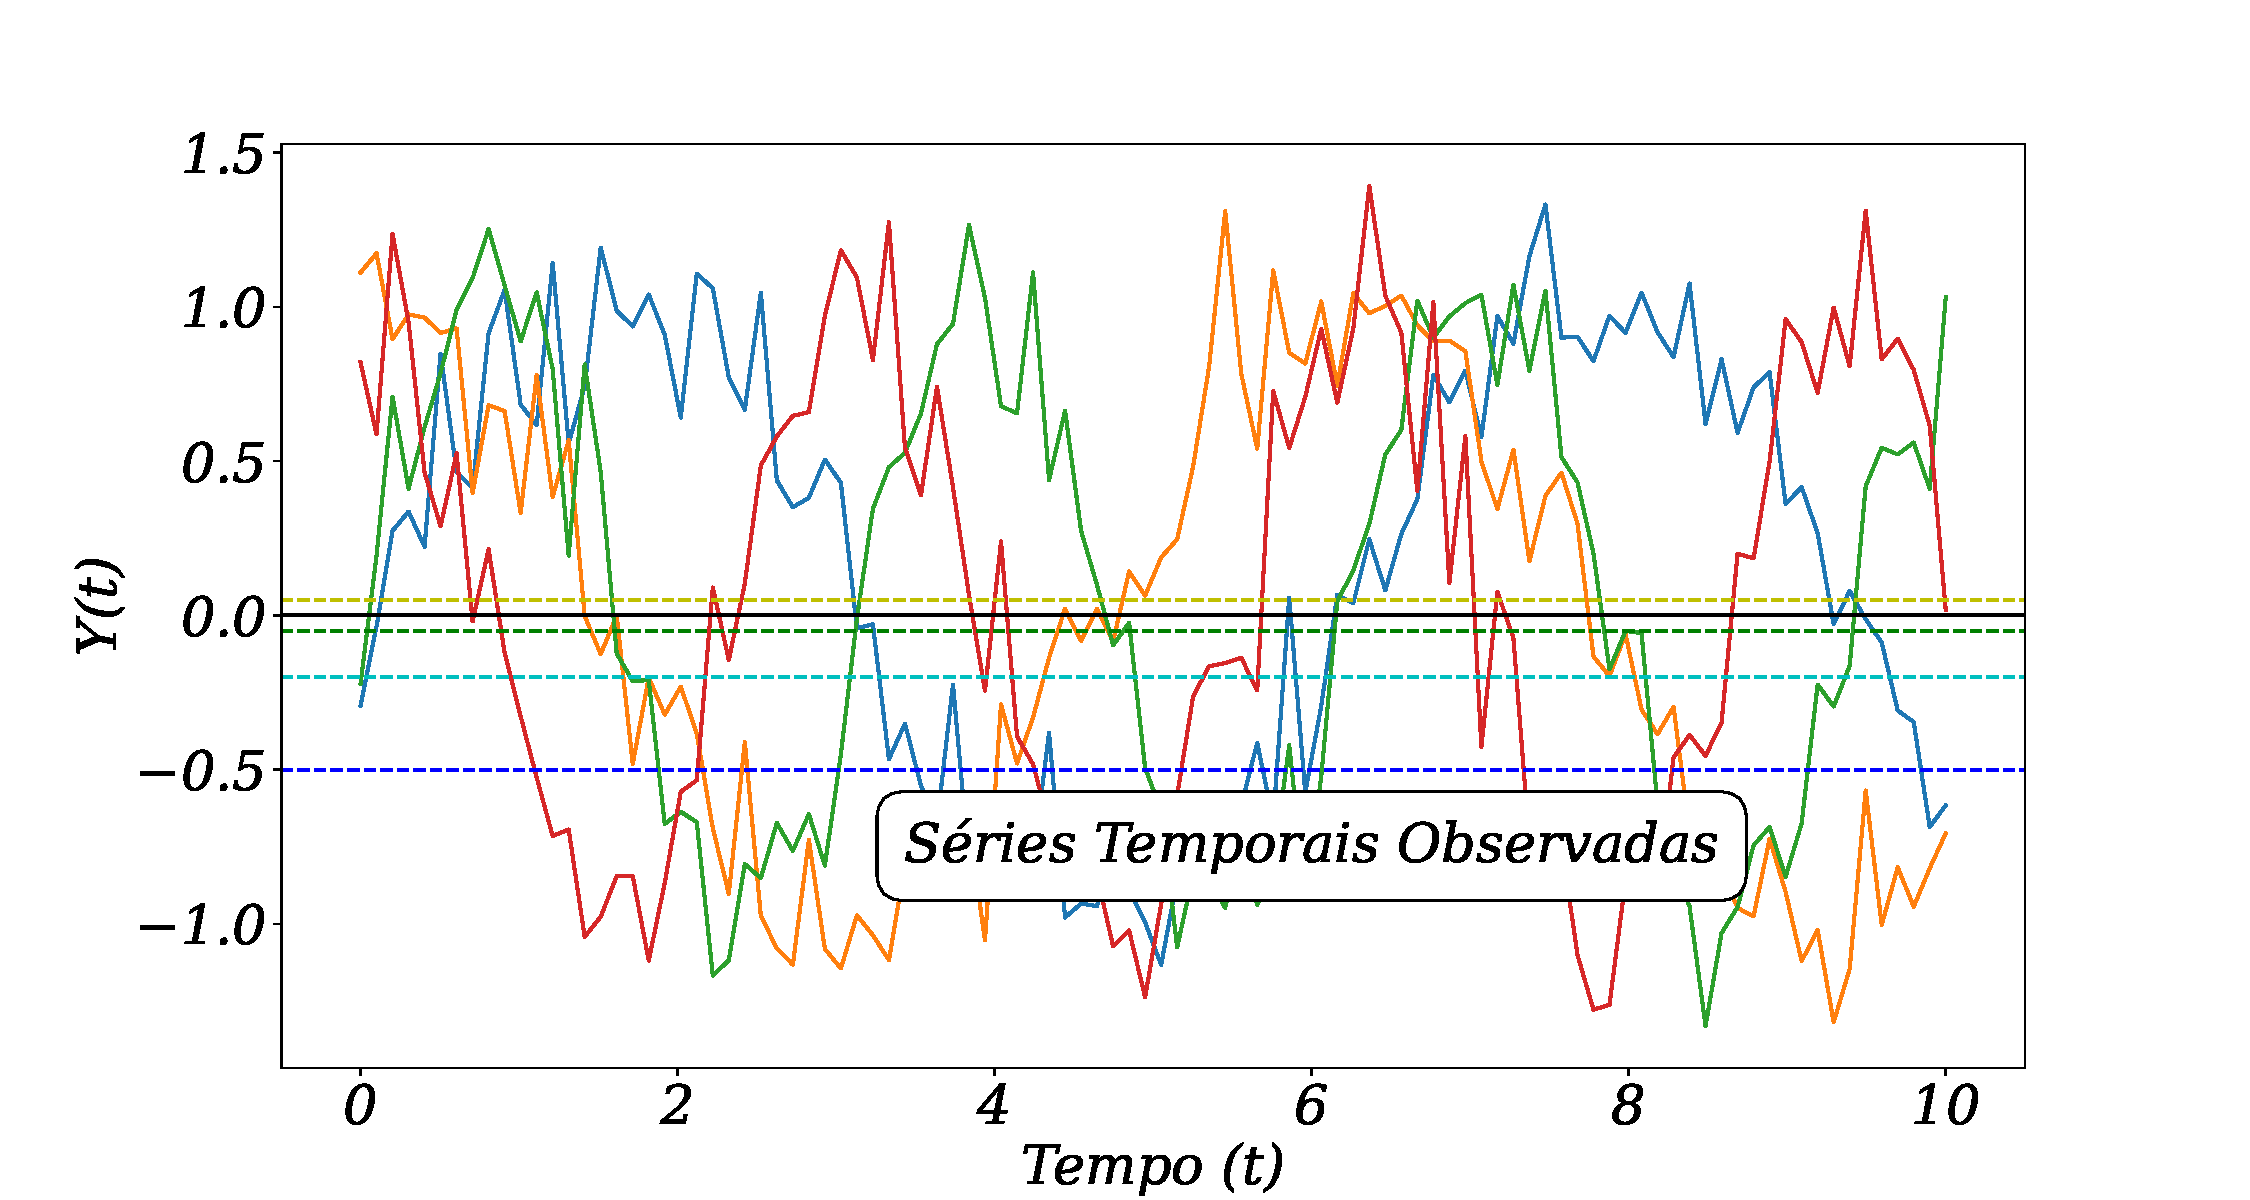
\includegraphics[width=1\linewidth]{Revisao/Figuras/serie}
	
	Fonte: \cite{pinheiro_2022}
\end{figure}

Com $Y(t)$ sendo os dados ficticiosos e $Tempo \ (t)$ a linha do tempo da Figura \ref{fig:serie}.

De repente é pensado como um conjunto de todas as possíveis trajetórias que poderia ser observar uma variável.


Essa revisão sistemática da literatura, com o tema abordado até o momento é sobre série temporal, considerando o contexto exposto aqui, esse tema pode ser de grande relevância em várias áreas tais como mostra na Figura \ref{fig:areas}. Realizar essa análise de série temporal ao longo de 6 últimos anos para poder observar os melhores feitos nesse tema, aborda aqui um curto período, mas tendo o tempo não muito a favor por isso tive a escolha de deixar esse tempo específico de busca de artigo.

Para essa revisão tem com objetivo a análise de uma literatura menor, porém bem relevante. Como a própria série temporal procura analisar e modelar dependência, e considerando a ordem apresentada nas bases, por exemplo, os maiores autores e o ano de atuação que eles, mais publicou nos países que tem o maior número de publicação, na apresentação das palavras chaves que será mostrado, o objetivo estar em rever cada coisa que pode ser usada em uma aplicação de aprendizado de máquina.

Em todos os artigos observar-se que tem uma contribuição científica, nesse trabalho é a análise de conceito de séries temporais com o melhor aproveitamento das palavras chaves, mesmo não tendo um grande relacionamento em aprendizado de máquina pode ser usado esses artigos como base para outros pesquisadores, sendo aqui algumas análises bem simples para alguns leitores. Entretanto é um ponto de partida para muitos que não conhece o conceito de série temporal ou revisão sistemática da literatura.


\subsection{Problematiza\c c\~ao da Revis\~ao} \label{subsec: problematização da revisão}

Nessa seção é abordado um problema de pesquisa que pode ser entendido por vários leitores, na Figura \ref{fig:serie-temporal} é apresentado um mapa conceitual de publicação e os autores são o pilar mais relevante para a revisão pois eles apresenta vários modelos que servira de base, e como está falando de série temporal a previsão que pode ser realizado nesse contexto é uma problemática devidamente de grande significância.

\begin{figure}[H]
	\centering
	\caption{Mapa conceitual do problema de pesquisa.}
	\label{fig:serie-temporal}
	\includegraphics[width=1\linewidth]{Revisao/Figuras/"Série temporal"}
	
	Fonte: Elaboração própria 
\end{figure}

No mapa conceitual apresentado na Figura \ref{fig:serie-temporal} é visto a problemática sendo relacionada com palavras, deixando evidente o que vai ser abordar no decorrer do trabalho deixando as questão de pesquisa em tópicos, logo adiante.

\begin{enumerate}[start=1, label = {\textbf{Q} \arabic* } ]
	\item \label{questão:rev1}Quais os autores que mais pública sobre o assunto de série temporal?
	\item \label{questão:rev2}Quais os países que mais pública sobre o assunto? 
	\item \label{questão:rev3}Quais as áreas que mais pública sobre o tema?
	\item \label{questão:rev4}Quais são as obras mais influentes na análise de séries temporais?
\end{enumerate}

\subsection{Metodologia}\label{subsec:met da revisão}

Nessa seção é esclarecido como foi conduzindo a revisão, desde analise das bases de dados até como concluir a revisão.

\begin{figure}[H]
	\centering
	\caption{Etapas da Revisão.}
	\label{fig:rsl}
	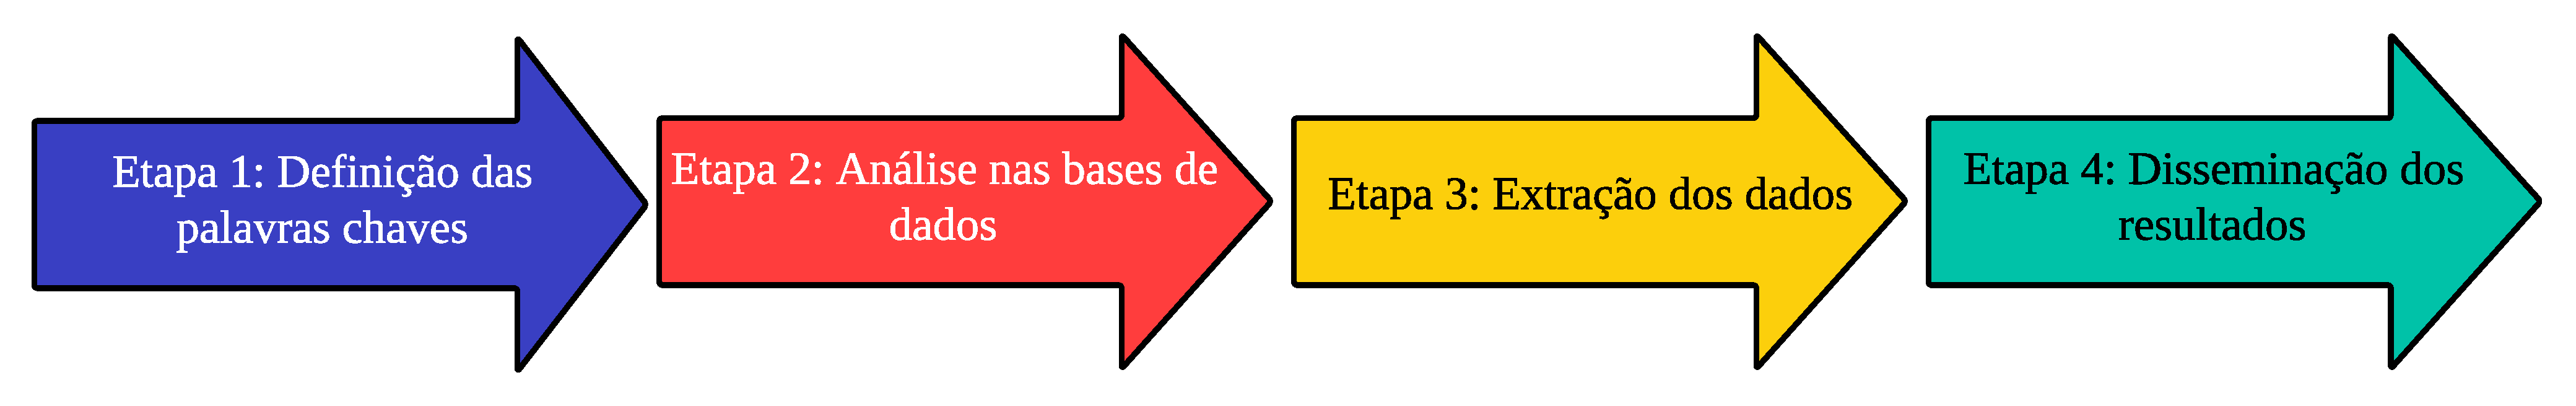
\includegraphics[width=0.7\linewidth]{Revisao/Figuras/RSL}
	
	Fonte: Adaptado de \citeonline{MARTINS201671}
\end{figure}
\begin{enumerate}[start=1, label = {\textbf{Etapa} \arabic* } ]
\item \label{etp:rev-1}Na Figura \ref{fig:rsl} usa uma adaptação de \citeonline{MARTINS201671} para essa revisão sistemática que esta sendo analisado. Logo mais tem as buscas nas bases da Scopus, Web of Science e Lens. A princípio foi usado algumas base no meio de tantas na literatura para melhor atende no tema da pesquisa.


\textbf{Campo de pesquisa Scopus}

\textbf{\textit{TITLE-ABS-KEY (``time series forecasting")  AND  TITLE-ABS-KEY (``time series analysis")  AND  ( LIMIT-TO ( DOCTYPE ,  ``ar" ) )  AND  ( LIMIT-TO ( LANGUAGE ,  ``English" ) )  AND  ( LIMIT-TO ( PUBYEAR ,  2022 )  OR LIMIT-TO ( PUBYEAR ,  2021 )  OR  LIMIT-TO ( PUBYEAR ,  2020 )  OR  LIMIT-TO ( PUBYEAR ,  2019 )  OR  LIMIT-TO ( PUBYEAR ,  2018 )  OR  LIMIT-TO ( PUBYEAR ,  2017 ) )}}

\textbf{Campo de pesquisa na Web of Science}

\textit{\textbf{``times series forecasting" (All Fields) and ``time series analysis" (All Fields)}} (Publication Years: 2022 or 2021 or 2020 or 2019 or 2018 or 2017) (Document Types: Articles) (Languages: English)

\textbf{Campo de pesquisa de Lens}

\textit{\textbf{Scholarly Works (11) = ( ``time series forecasting" ) AND ( ( ``time series analysis" ) AND ( ``nonlinear forecasting" ) ) }}
Filters: Year Published = ( 2016 - 2022  ) Publication Type = ( journal article  )\\


Em todos os campos de busca realizado nos últimos 6 anos, apenas no site do lens que optou-se para colocar 6 anos, pois nos retornou poucos artigos. Nessa etapa é usado as palavras chaves que mais se adéquam na pesquisa \textit{time series forecasting and time series analysis and nonlinear forecasting}.

	\item \label{etp:rev-2} No cruzamento de palavras obter um número considerável de artigos sem restringir a área que cada artigo pode estar publicado. Na Tabela \ref{tb1} foi realizado um tabelamento dos resultados obtidos sem excluir a duplicada, isso vamos tratar na seção \ref{subesec:resul da revisão}.

\item \label{etp:rev-3}Essa etapa serve para avaliar cada dado que obter sem nenhum filtro no começo da pesquisa, a extração desses dados sem usar nenhum filtro de ano nas buscas, ficaria muitos artigos para analisar, como por exemplo, na base de dados da Scopus ficaria com $498$ artigos, na Web of Sceince ficaria com $140$ artigos, e no Lens como não retornara muitos artigos, fica com $11$ dando em um total de $649$ sem remover duplicada. É certo lembrar que nesses artigos tem somente o filtro do idioma inglês e de artigo, para melhora a busca e tomada de decisão usando o filtro de anos, nos últimos 6 anos é um valor de artigos mais agradável de ser utilizado com pouco tempo para analisar, e usar a diferença ente essa estimativa que foi realizado na Tabela \ref{tb1} são menos de $ 356 $ artigos para analisar. Lembrando que se foi feito a remoção dos duplicados esse número que foi obtido no resultado das bases todas pode chegar a um número menos ainda do que é pretendido nesse trabalho.

\item  \label{etp:rev-4}Nessa etapa é mais para analisar a dimensão do que está sendo trabalhado, fazendo a análise das áreas e ler os artigos que são realmente importantes para a revisão. Como essa revisão é voltado a séries temporais em um programa de mestrado de engenharia de produção e sistemas é valido analisar a correlação. Dessa forma um das áreas é voltado a matemática assim sendo selecionado nesses artigos que pode ter um resultado de uma análise mais profunda dos artigos de séries temporais, se olhar para as áreas de atuação dos artigos pesquisados pode ser visto na Figura \ref{fig:areas} que as áreas que foi citado aqui com grande relevância é \textbf{informática, engenharia e matemática} tem um número de publicação bem elevado, representando $50\%$ da busca, então a pesquisa esta no caminho certo, usando a matemática básica para ter uma estimativa de quantos artigos pode ser eliminado seria por volta de $481$ artigos, mas isso sem muito fundamento de que esse número tenha uma precisão. Usando o \textit{software mendeley desktop}  para estipular o valor exato de quantos artigos usar, sem duplicado fica com um número de $308$ artigos.
\end{enumerate}

\subsection{Resultados da busca da revis\~ao}\label{subesec:resul da revisão}


Nessa seção vai ser apresentado os resultados da pesquisa usando alguns \textit{softwares} para conseguir estipular o melhor aproveitamento de cada base de dados usado no decorrer do trabalho. Dessa forma pode começar com a análise no \textit{software VOSviewer} 

\begin{figure}[htp!]
	\centering
	\caption{Palavras-chave mais populares na Scopus.}
	\label{fig:scopus-09-08}
	\includegraphics[width=0.9\linewidth]{Revisao/Figuras/"scopus 09-08"}
	
	\vspace{0.2cm}
	Fonte: Elaboração própria a partir de dados da Scopus (2016 a 2022)
\end{figure}
Na Figura \ref{fig:scopus-09-08} é uma relação das palavras mais utilizadas como sinônimos da palavra \textit{time series analysis}, ou em conjunto no corpo do texto dos artigos.
A análise da base de dados na scopus foi feita na ferramenta que mostra as palavras chaves que pode ser relacionado em todo campo de pesquisa, com isso tem uma ampla visão do que pode ter correlação com as palavras-chave mãe da pesquisa.

Na relação entre as palavras chaves nesse primeiro momento, obteve um resultado de 3484 palavras-chave, 212 cumprem o limiar, lembrando que as palavras de base para resultar foi \textit{time series forecasting and time series analysis } na Scopus.

\begin{figure}[htpb!]
	\centering
	\caption{Palavras-chave mais populares na Web of Science}
	\label{fig:web-09-08}
	\includegraphics[width=0.8\linewidth]{Revisao/Figuras/"web 09-08"}
	
	
	
	\fonte{Elaboração própria a partir de dados da Web of Science (2016 a 2022)}
\end{figure}


Na Figura \ref{fig:web-09-08} a análise da base de dados na Web of Science foi feita na ferramenta que mostra as palavras chaves que esta relacionado em todo campo de pesquisa, com isso pode ter uma ampla visão do que tem correlação com as palavras-chave mãe da pesquisa.

Na relação entre as palavras chaves nesse primeiro momento, teve um resultado de 305 palavras-chave, 13 cumprem o limiar, lembrando que as palavras de base para resultar foi \textit{time series forecasting and time series analysis } na web of science.


A única base de dados que não sera mostrado aqui é a base da Lens, pois a mesma sendo uma base ótima ainda não teve tanto retorno na pesquisa que foi feito. O site lens retornou apenas 11 artigos com os filtros aplicados. Na \ref{etp:rev-1} é observado o campo de busca que foi utilizado nessa pesquisa que deu 11 artigos somente.


\begin{table}[htpb!]
	\caption{Cruzamento de palavras-chave através da aplicação de filtros de ano e de linguagem}\label{tb1}
	\centering
	\begin{tabular}{@{}cp{2cm}p{1cm}p{2cm}p{1cm}p{2cm}p{2cm}p{2cm}@{}}
		\toprule
		Bases                             & \multicolumn{5}{c}{Palavras Chaves}                                                         & Resultado \\ \midrule
		\multirow{2}{*}{Scopus}           & time   series forecasting & AND & time   series analysis    &     &                         & 490       \\
		& nonlinear forecasting     & AND & time   series forecasting &     &                         & 8         \\
		\multirow{2}{*}{Web   of Science} & time   series forecasting & AND & time   series analysis    &     &                         & 126       \\
		& nonlinear forecasting     & AND & time   series forecasting &     &                         & 14        \\
		Lens                              & time   series forecasting & AND & time   series analysis    & AND & nonlinear   forecasting & 11        \\
		\multicolumn{6}{c}{Total}                                                                                                       & 649       \\ \bottomrule
	\end{tabular}
	
	\fonte{Elaboração própria a partir de dados da Scopus, Lens e Web of Science (2016 a 2022)}
\end{table}


Na Tabela \ref{tb1} relaciona as palavras chaves para cada base e aumenta a quantidade de artigo em todas as bases, mas essa Tabela esta com os dados brutos que não foi eliminado os duplicados, então usando o \textit{software mendeley} para remoção dos duplicados retorna apenas  308 artigos.




\begin{figure}[htp!]
	\centering
	\caption{Analise das quantidades de artigos em relação aos anos.}
	\label{fig:regressao-linear-dos-artigos-baseados-nos-anos}
	\includegraphics[width=0.9\linewidth]{Revisao/Figuras/"regressão linear dos artigos baseados nos anos"}
	
	\fonte{Elaboração própria a partir de dados da SANEPAR (2018 a 2020)}
\end{figure}

A Figura \ref{fig:regressao-linear-dos-artigos-baseados-nos-anos} tem com abscissa e ordenada, anos e artigos sendo assim a relação entre a data de publicação dos artigos no decorrer do tempo.

Número considerável de artigo para analisar, na Figura \ref{fig:regressao-linear-dos-artigos-baseados-nos-anos} foi feito uma análise baseado em uma regressão linear dos artigos em decorrer dos anos desde 2016 até 2022 nessa análise obteve a seguinte equação de regressão linear:

\begin{eqnarray}
	y(x)&=&8,3571x - 16803 \qquad \text{Com } R^2=0,3062\label{eq1}
\end{eqnarray}

Sendo $y(x)$ a equação da reta na equação \eqref{eq1}. $8,3571$ é o coeficiente angular do gráfico de $ y(x) $ $16.803$ é o coeficiente linear, ou o ponto de intersecção com o eixo $y$, $x$ é a variável independente.

Este coeficiente indica a proporção da variância da variável dependente que pode ser estatisticamente atribuída ao conhecimento de uma ou mais variáveis independentes \citeonline{coeficiente}. 

O coeficiente de determinação mensura a relação existente entre a variável dependente e as variáveis independentes, indicando qual o percentual de variação explicada pela regressão, representa da variação total. Quando:

$R^2=1$: todos os pontos observados se situam exatamente sobre a reta de regressão (ajuste perfeito), ou seja, as variações de $y$ são $100\%$ explicadas pela variação dos $x_n$ através da função especificada, não havendo desvios em torno da função estimada. 

$R^2=0$: conclui-se que as variações de $y$ são exclusivamente aleatórias e a introdução das variáveis $x_n$ no modelo não incorporará informação alguma sobre as variações de $y$.

\begin{equation}
	R^{2}=\frac{\left(\sum X . Y-\frac{\sum X \cdot \sum Y}{n}\right)^{2}}{\left[\sum X^{2}-\frac{\left(\sum X\right)^{2}}{n}\right] \cdot\left[\sum Y^{2}-\frac{\left(\sum Y\right)^{2}}{n}\right]}=(r)^{2}\label{eq2}
\end{equation}

Na equação \eqref{eq2} $X,Y$ é dado pelas coordenadas no plano cartesiano, como por exemplo o par ordenado $(x,y)$. 
Na equação \eqref{eq1} observa-se que obteve o $R^2=30\%$ isso acarreta que a reta de regressão será influenciada pelo $R^2$ que foi achado.

Apesar de ser uma análise bem simples que foi realizada com a relação entre quantidade de artigos e anos, ainda sim e uma ótima validação de se olhar no teste de significância F que é dado a significância tem que estar sempre $F<5\%$ esse teste também é chamado valor-p (p-value).

Tendo esses valores pode ser analisado a extrema significância, na reta de regressão observar-se que em 2021 foi o ano que mais foi publicado artigos com esse tema de séries temporais, essa analise pode nos trazer o pico maior de publicação feito.

\begin{table}[H]
	\centering
	\caption{Fator de impacto}\label{tb2}
	\begin{tabular}{@{}cp{3cm}p{3cm}c@{}}
		\toprule
		Revista cientíica      & Quantidade de plubicação & Qualidade da revista & H-INDEX \\\midrule
		Neurocomputing         & 27                         & Q1                     & 143     \\
		IEEE Access            & 18                         & Q1                     & 127     \\
		Applied Soft Computing & 12                         & Q1                     & 143     \\
		Energies               & 11                         & Q2                     & 93      \\
		Energy                 & 11                         & Q1                     & 343     \\ \bottomrule
	\end{tabular}
	
	
	\fonte{Elaboração própria a partir de dados da Scopus, Lens e Web of Science (2016 a 2022)}
\end{table}


Na Tabela \ref{tb2} mostra algumas revistas que mais pública, artigos nesse tema, como muita revista não se localiza no Brasil tem o nome em inglês, mas todas as revistas com um fator de impacto bem elevado como \textbf{A1} tem uma correlação com as áreas de \textbf{informática, engenharia e matemática}.

\begin{figure}[htpb!]
	\centering
	\caption{Relação de autores entre artigos publicados}
	\label{fig:autores-relacao-entre-artigos-publicados}
	\includegraphics[width=0.8\linewidth]{Revisao/Figuras/"Autores Relação entre artigos publicados"}
	
	
	\fonte{Elaboração própria a partir de dados da Scopus (2016 a 2022)}
\end{figure}

\begin{figure}[htpb!]
	\centering
	\caption{Ligação bibliográfica entre os autores}
	\label{fig:autores}
	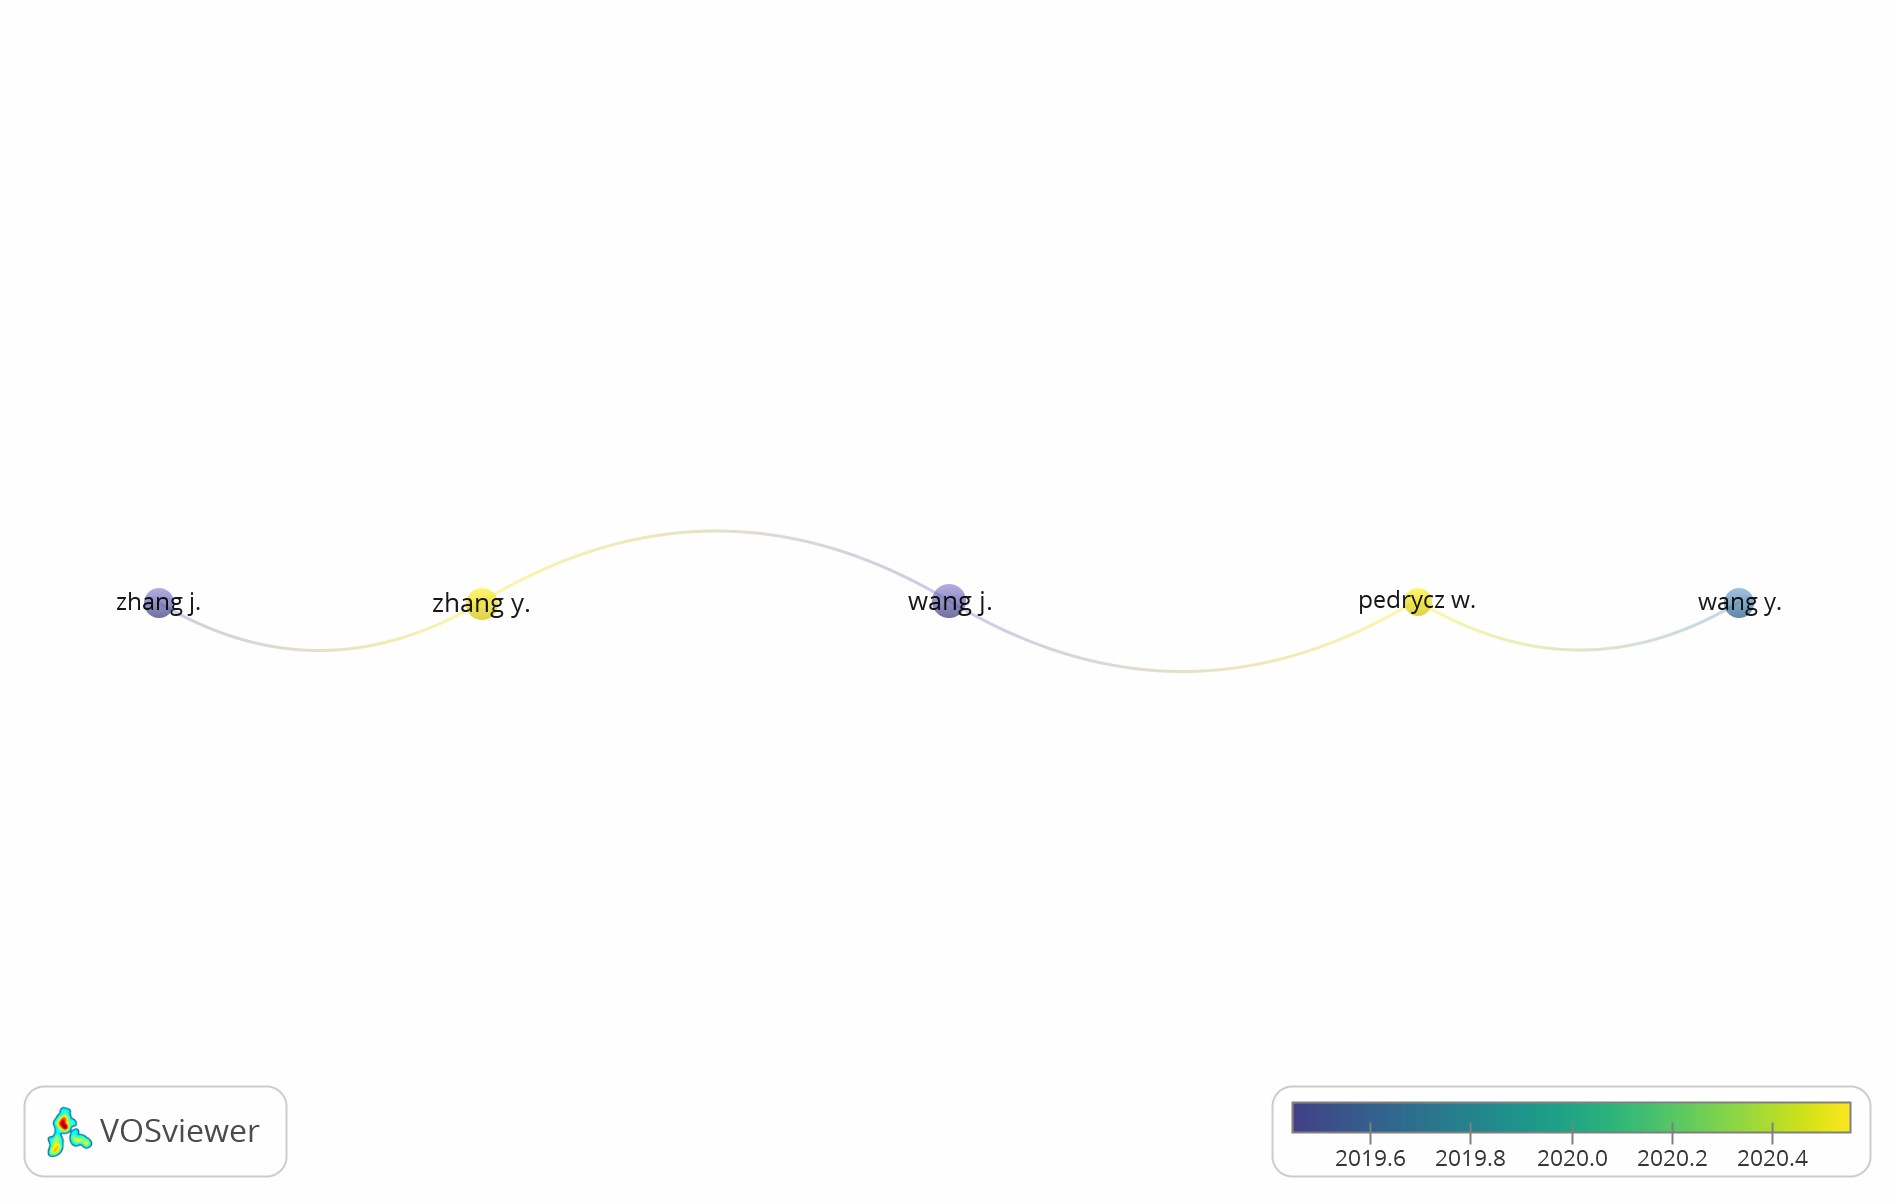
\includegraphics[width=0.8\linewidth]{Revisao/Figuras/Autores}
	
	\fonte{Elaboração própria a partir de dados da Scopus (2016 a 2022)}
\end{figure}


 Respondendo um problema de questão feito aqui a \ref{questão:rev1} utiliza a Figura \ref{fig:autores-relacao-entre-artigos-publicados} com um gráfico de histograma, como que fique mais visível os autores que mais pública nesse tema, no gráfico coloca os autores que tiveram publicação maior que 4, e com isso não coloca todos os autores, levando em consideração os autores que publicaram acima de 4 artigos nesse tema de 2016 até 2022.

\begin{figure}[htpb!]
	\centering
	\caption{Mapa mundial da publicação de artigos em todo o mundo}
	\label{fig:mapa-mundi-artigos}
	\includegraphics[width=1\linewidth]{Revisao/Figuras/"mapa mundi artigos"}
	\vspace{0.2cm}
	
	\fonte{Elaboração própria a partir de dados da Scopus, Lens e Web of Sicence (2016 a 2022)}
\end{figure}



Na questão de pesquisa \ref{questão:rev2} é respondia com a Figura \ref{fig:mapa-mundi-artigos}, os país que mais pública sobre o assunto, em escala de maior publicação para o menor em escalar da seguinte forma China - 119, Estados Unidos - 67, Índia - 57, Brasil - 32, Espanha - 28, Reino Unido - 25, Austrália - 24, Irã - 18, Malásia - 17, Canadá - 16. No mapa não aparece todos os países com seus números de publicações.


\begin{figure}[htpb!]
	\centering
	\caption{Áreas de aplicação do tema}
	\label{fig:areas}
	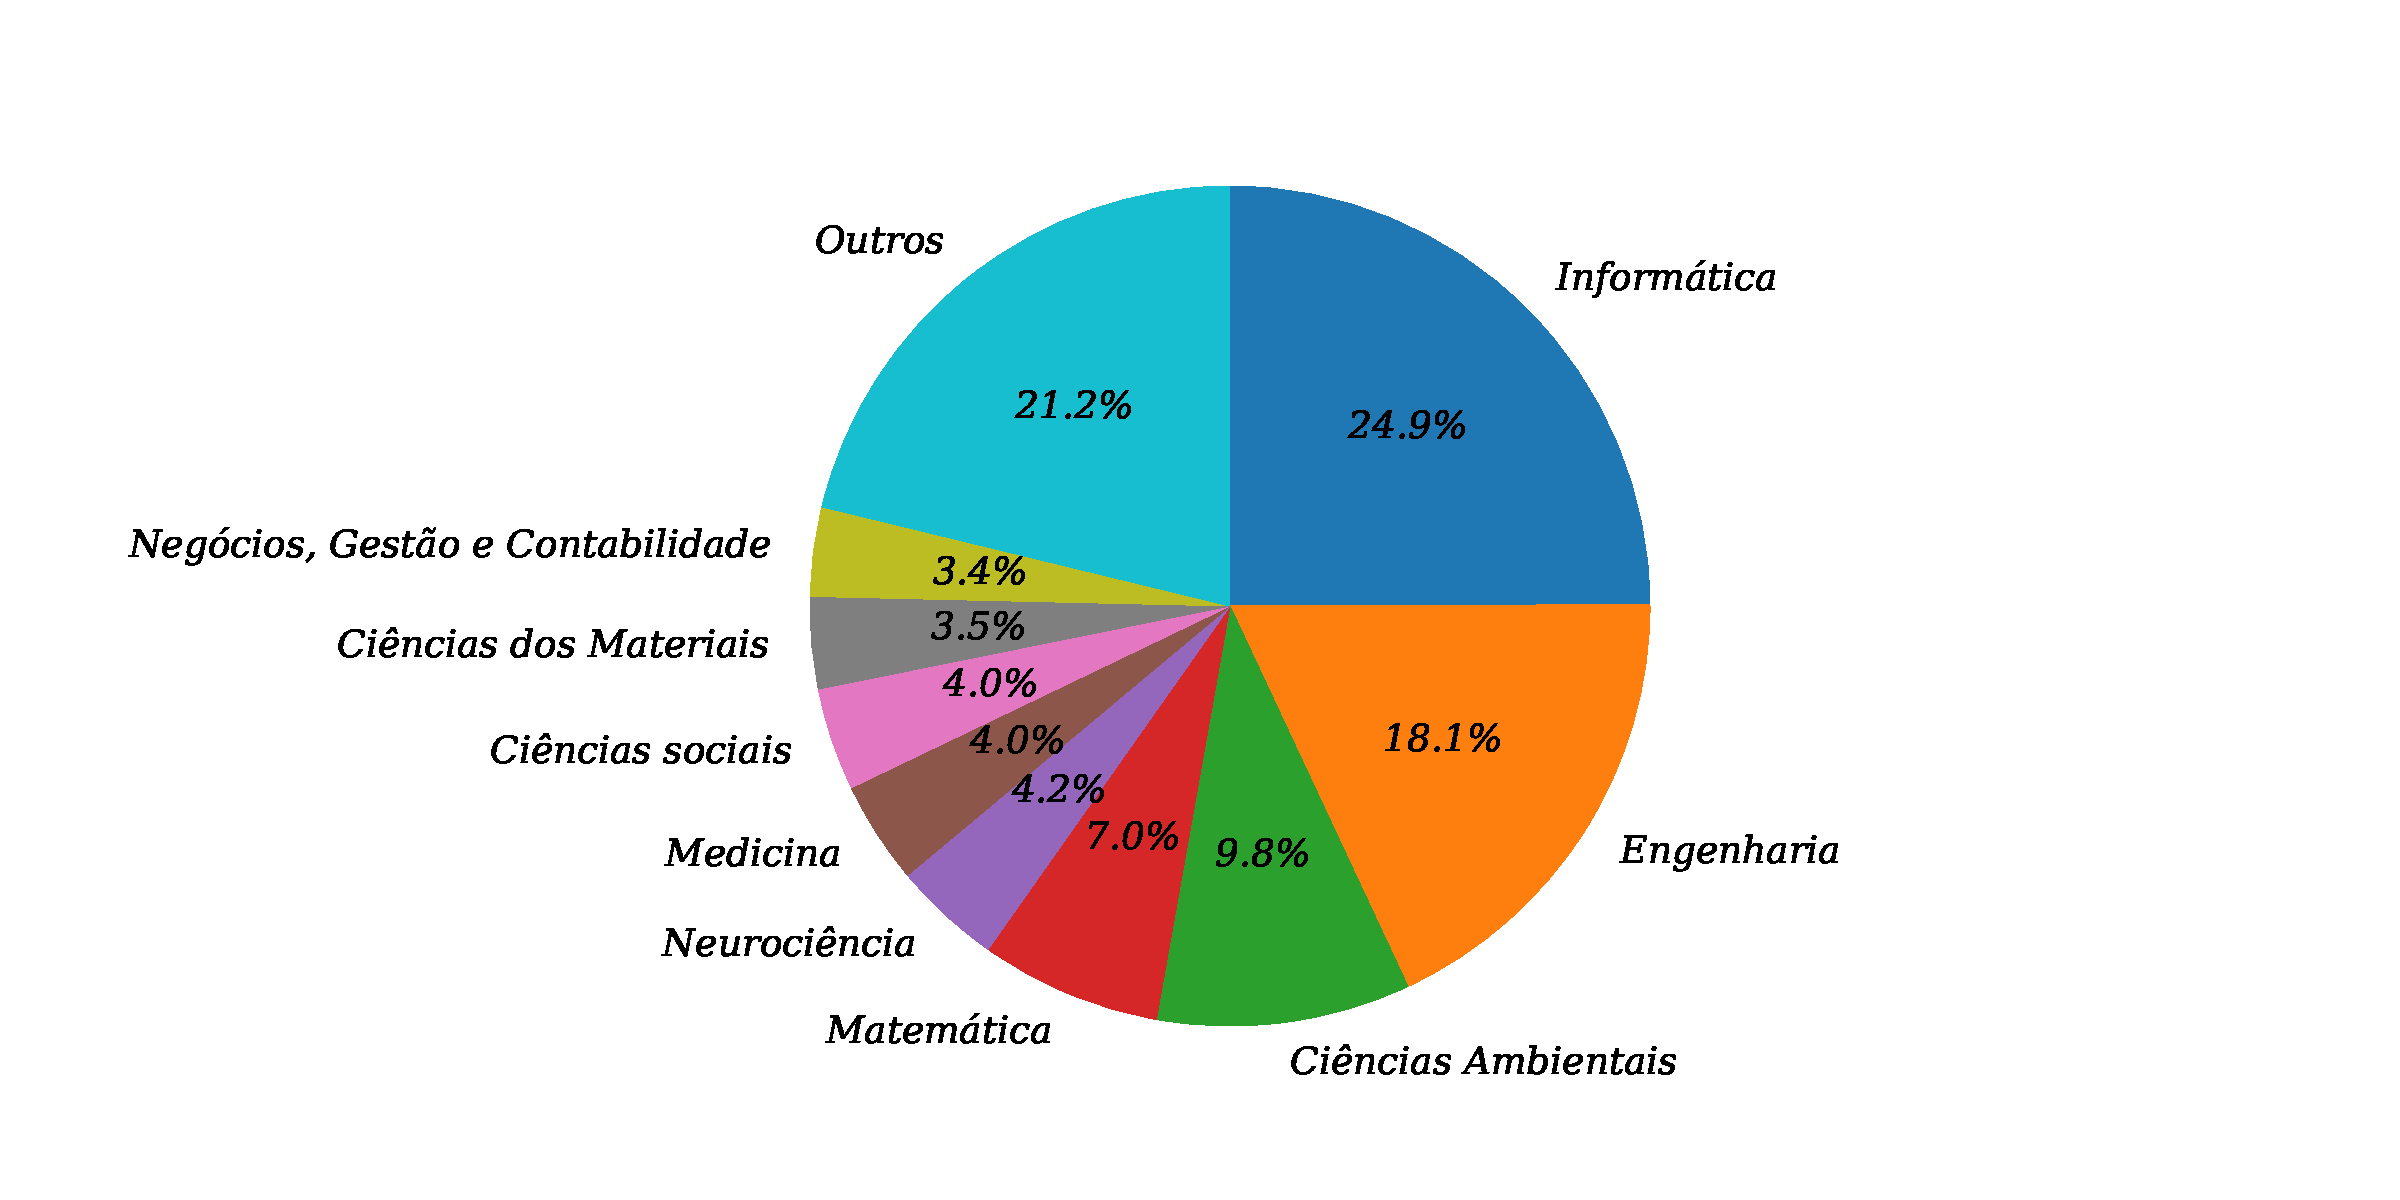
\includegraphics[width=0.9\linewidth]{Revisao/Figuras/areas}
	\vspace{0.2cm}
	
	\fonte{Elaboração própria a partir de dados da Scopus, Lens e Web of Sicence (2016 a 2022)}
\end{figure}


Questão de pesquisa \ref{questão:rev3} para responder essa questão foi feito um gráfico circular de modo a rotular as áreas que mais tem publicação no tempo escolhido na revisão. Na Tabela \ref{tb3} mostra os valores de cada área e sua quantidade de publicação. 

\begin{table}[!htb]
	\centering
	\caption{Áreas e seus valores respetivos de artigos em cada área.}\label{tb3}
	\begin{tabular}{@{}ll@{}}
		\toprule
		Informática                      & 240 \\ \midrule
		Engenharia                       & 174 \\
		Ciências Ambientais              & 94  \\
		Matemática                       & 67  \\
		Neurociência                     & 40  \\
		Medicina                         & 38  \\
		Ciências sociais                 & 38  \\
		Ciências dos Materias            & 34  \\
		Negócios, Gestão e Contabilidade & 33  \\
		Outros                           & 204 \\ \bottomrule
	\end{tabular}

	
	\fonte{Elaboração própria a partir de dados da Scopus, len e Web of Sicence (2016 a 2022)}
\end{table}
	



Na última questão \ref{questão:rev4} de pesquisa foi feito um levantamento de alguns dos artigos mais influentes da revisão esses artigos retrata de alguns métodos sobre séries temporais os artigos dos autores \citeonline{Golyandina2020, Kumar2021, Xie2019, Lara-Benitez2021, Ahmad2018, CarvalhoJr.2019, Tan2021, Liu2019, Liu2021, Rossi2018, Soyer, Martinovic2020a, Ursu2016, Wang2016, Shih2019a, Moon2019, Chou2018, Bergmeir2018, Boroojeni2017, Chou2018a, Coelho2017, Du2020, Sadaei2019, Salgotra2020, Tyralis2017, Vlachas2020, Yang2019a, Shen2020, Sezer2020, Chen2018, Buyuksahin2019, Li2020, Kulshreshtha2020, Samanta2020, Xu2019, Graff2017, Taieb2016}
 alguns métodos utilizado pelos autores para previsão de séries temporais, e alguns modelos de análise do mesmo, previsão não linear. 
 
 \citeonline{Xu2019} no modelo híbrido, o modelo linear AR e LR ou o modelo ARIMA e o modelo DBN não linear são explorados para captar os comportamentos lineares e não lineares de uma série temporal, respectivamente. \citeonline{Li2020} o desempenho de previsão da abordagem MAELS é comparado aos predecessores baseados na aprendizagem de máquinas do estado para a arte, tais como CNN, RNN, LSTM, ARIMA, e SVM-VAR. As abordagens, CNN, RNN e LSTM permitem o tratamento de entrada e saída multivariada, o ARIMA utiliza dados passados para prever o futuro, usando dois principais recursos: a autocorrelação e médias móveis.

Então com essa revisão sistemática e análise do conteúdo obteve a resposta da responder à questão de pesquisa feita no começo do capítulo, com essa revisão sistemática pode perceber haver muitos métodos em séries temporais.

Fora esses modelos também tem a atualização do ARIMA, que vai ser utilizado nessa dissertação, como SARIMA, SARIMAX, ambos desses modelos vai ser comparado para obter o melhor modelo entre eles, fora esse também sera utilizado o Light GBM e XGBoost. Para as métricas de erros nessa dissertação será utilizado as seguintes métricas e explicado no capitulo \ref{sec:base} MAE, MAPE e RMSE, na literatura é uma das mais usadas entre várias, com por exemplo o $R^2$ citado \eqref{eq2} para as previsões futuras sempre foi deparado com essas métricas de erros. o $R^2$ não é tão utilizado para comparação.

\subsection{Conclus\~ao da revis\~ao} \label{subsec:conclusão da revisão}

Nessa seção relatar o que foi abordado durante a pesquisa de revisão sendo ela em algumas bases como Scopus, Web of Science e Lens, cada base retornou vários artigos que foi analisado e com isso responde à questão de pesquisa feita na revisão, a pesar da base Lens foi a menor entre todas ainda encontra alguns artigos que foi de relevância no processo da dissertação, também com ajuda dos \textit{softwares} para analisar muitos arquivos e suas relações entre cada um. Séries temporais sendo uma análise profunda e mais atual na revisão sistemática, fazendo a busca nos 6 últimos anos.

Na busca realizada foi obtido alguns resultados bem relevante, como no cruzamento das palavras em cada base com o filtro aplicado obteve $ 308 $ artigos de $ 2016 $ até $ 2022 $, com isso foi preciso filtrar mais sobre cada área de atuação dos artigos, como matemática, engenharia e informática nesse filtro teve um total de $ 481 $ artigos excluindo que seria das outras áreas.




